\documentclass{beamer}
\usepackage[utf8]{inputenc}

\author[Sowmya Vajjala]{Instructor: Sowmya Vajjala}


\title[LING 120]{LING 120, Fall 2017: \\ Language and Computers}
\subtitle{Topic: Overview of Natural Language Processing}

\date{4 October 2017 (Week 7)}

\institute{Iowa State University, USA}

\usepackage{graphicx}
%%%%%%%%%%%%%%%%%%%%%%%%%%%

\begin{document}

\begin{frame}\titlepage
\end{frame}

\begin{frame}%2minutes
\frametitle{Class outline}
\begin{itemize}
\item Solution to yesterday's problem
\item Tasks in NLP: continuation
\item Midterm preparation time
\end{itemize}
\end{frame}

\begin{frame}
\frametitle{BrokEnglish! - solution}
\begin{itemize}
\item Problem: \url{http://www.nacloweb.org/resources/problems/2011/E.pdf}
\item Solution:\url{http://nacloweb.org/resources/problems/2011/ES.pdf}
\end{itemize}
\end{frame}


\begin{frame}
\frametitle{Madly Ambiguous: a web-game@OSU}
\url{http://madlyambiguous.osu.edu:1035/}
\end{frame}

\begin{frame}
\frametitle{NLP tasks: Parsing}
\begin{itemize}
\item Task: Construct the syntactic structure of a given sentence.
\item Two kinds of trees can be generated in NLP: Phrase structure tree (Constituency tree), Dependency tree
\item PST: shows parse structure in terms of Noun Phrases, Verb Phrases, Prep. Phrases etc.
\item Dependency Tree: shows relations between words in a sentence in terms of a pre-defined set of relations
\item Useful to develop various applications such as question-answering systems (like Siri)
\item Important note: POS tagging errors can carry over and affect parser efficiency. 
\end{itemize}
\end{frame}

\begin{frame}
\frametitle{NLP tasks: Parsing}
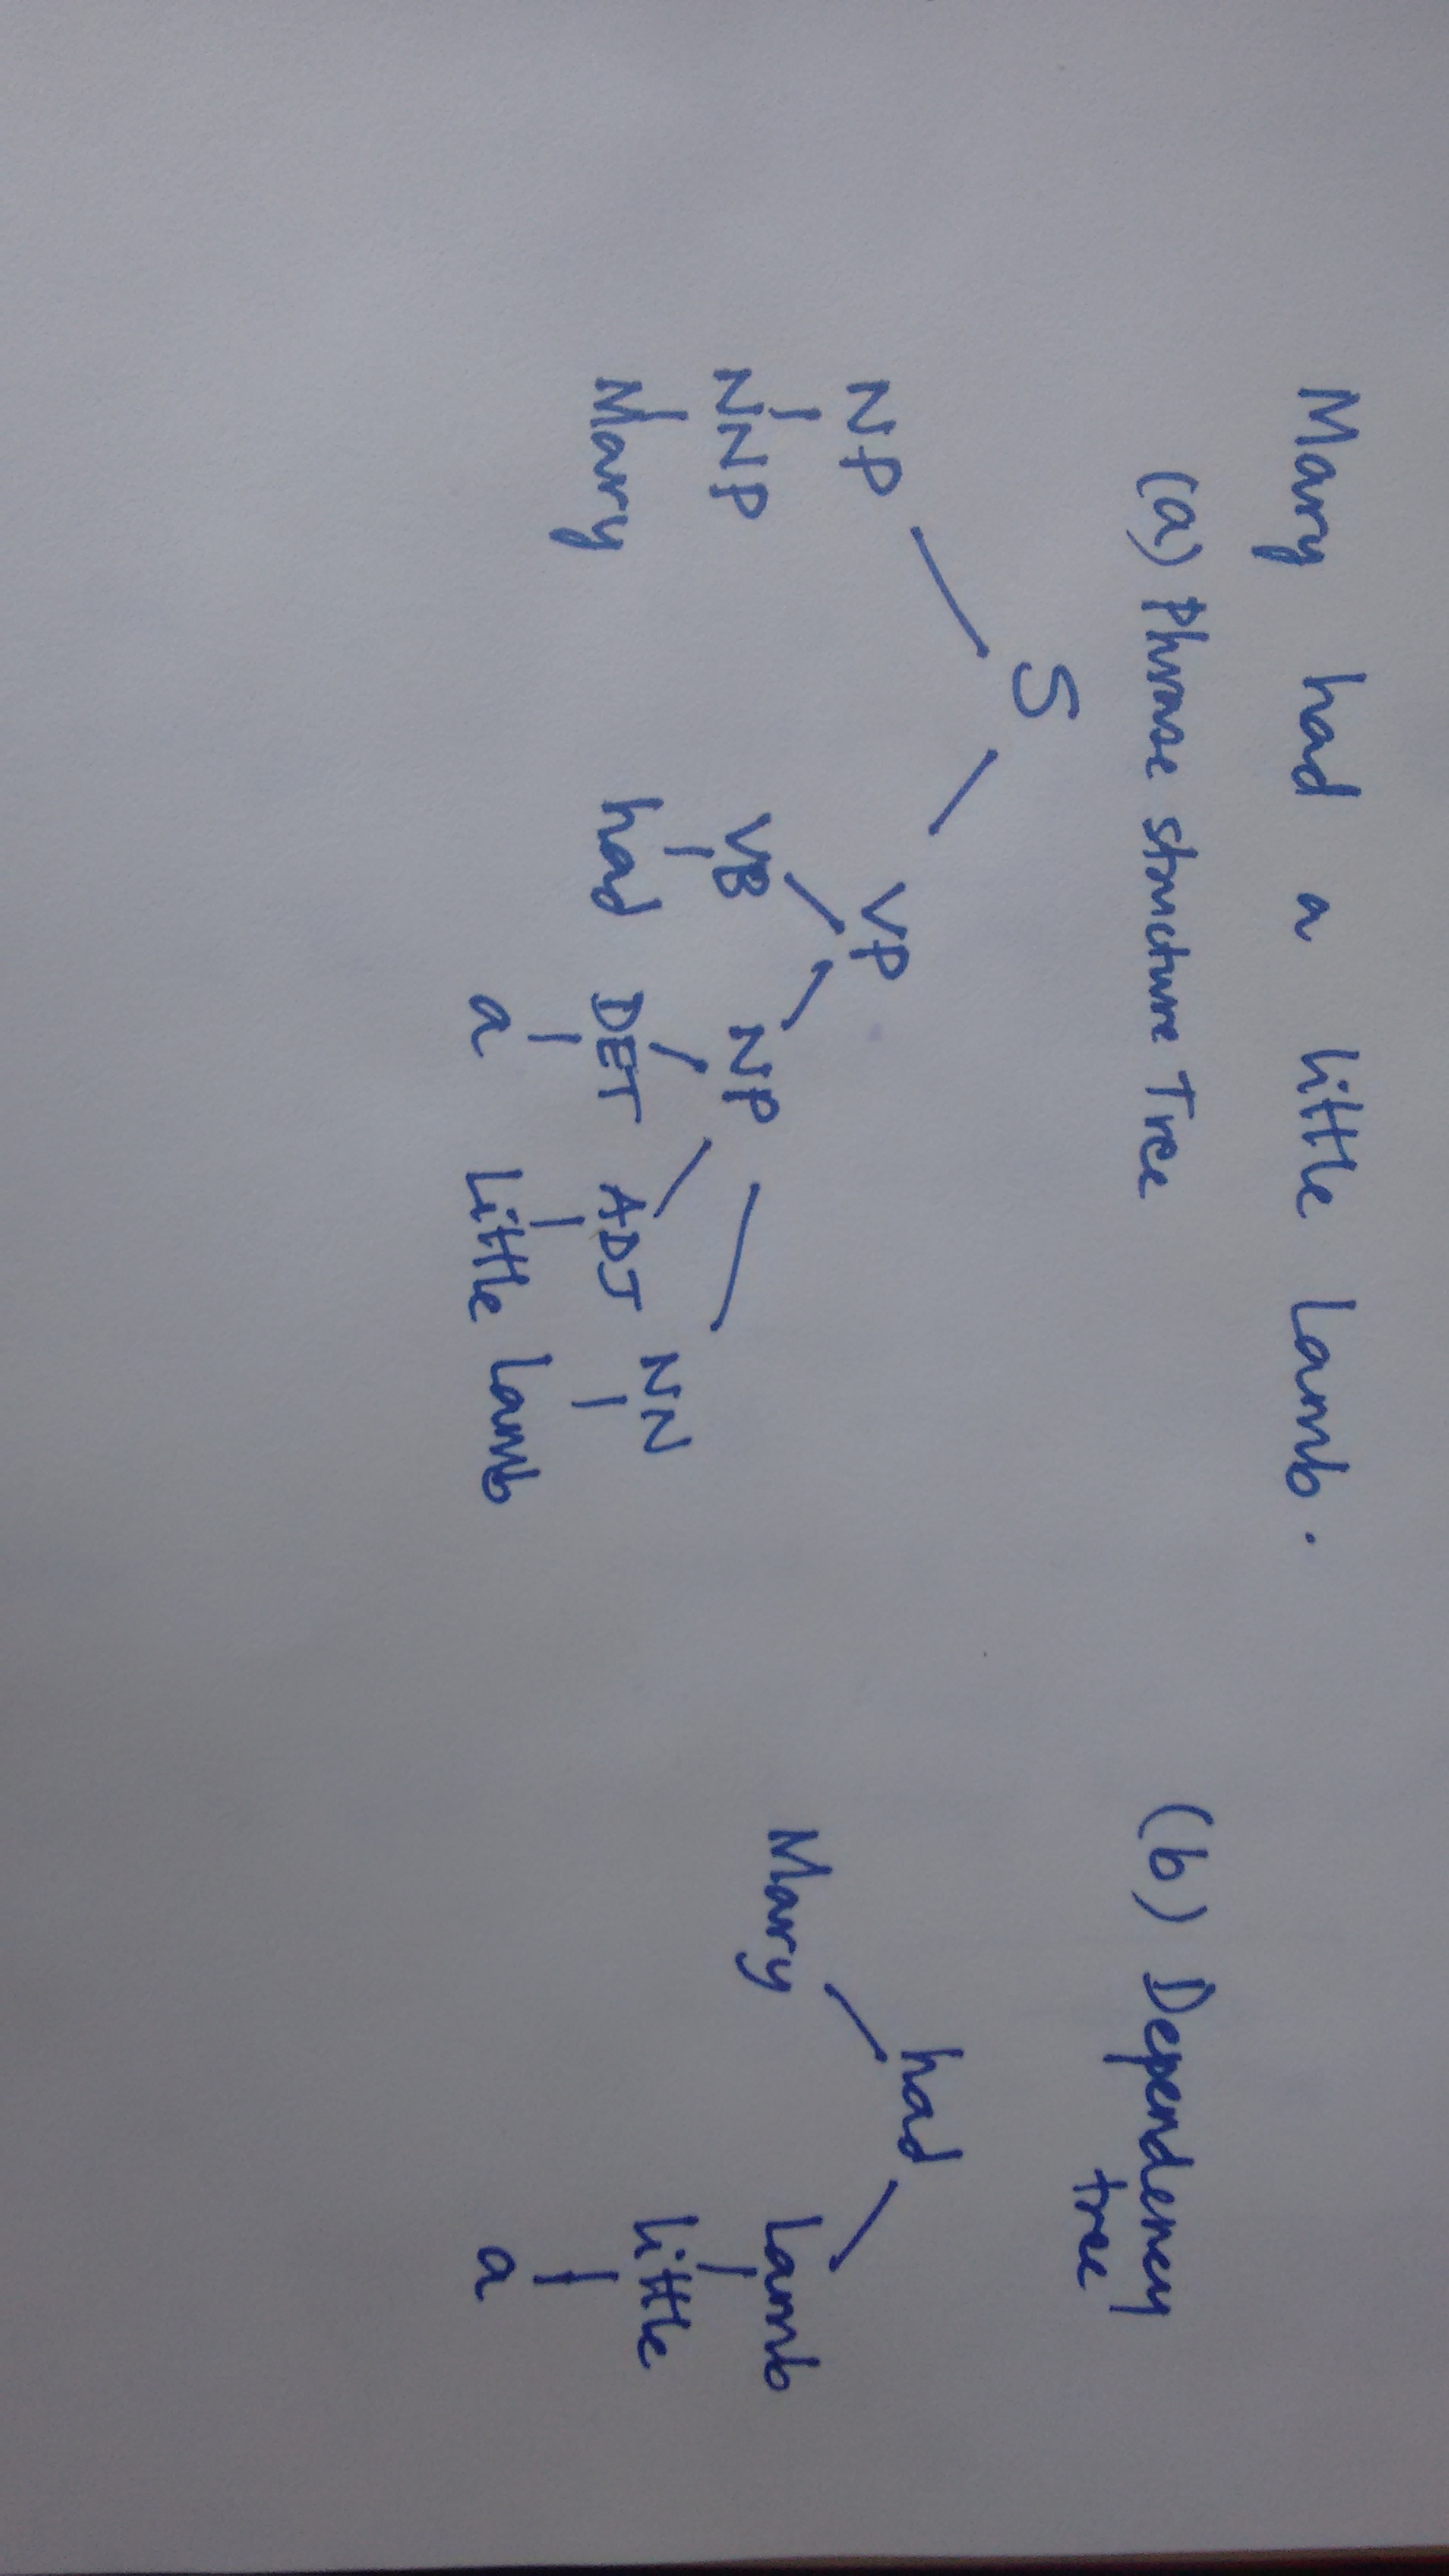
\includegraphics[width=0.6\textwidth,angle=90]{parses.jpg}
\\ \bigskip (to be continued)
\end{frame}

\begin{frame}
\frametitle{NLP tasks: Word Sense Disambiguation}
\begin{itemize}
\item Task: For words that can have multiple meanings, what is the right sense of the word in a given sentence? 
\item Example: "Let us go inside, it is cold" vs "I have cold and cough"
\item Very important for applications such as machine translation, information retrieval
\item Good progress for English WSD. One of the active areas of research in the field.
\end{itemize}
\end{frame}

\begin{frame}
\frametitle{NLP tasks: Named Entity Recognition}
\begin{itemize}
\item Task: Identify and classify named entities (e.g., person names, organization names, locations etc.,) 
\item Application: Information extraction from text 
\item Some NER is domain specific (biomedical NER, financial NER etc)
\item Current methods of NER: hand-crafted or automatically compiled lists + statistical machine learning models
\item Active area of research for English and other languages. 
\end{itemize}
\end{frame}

\begin{frame}
\frametitle{NLP tasks: Semantic Role Labeling}
\begin{itemize}
\item SRL is all about doing a "semantic parse" of a sentence. The task here is to identify argument structure of a sentence and thematic roles of different entities.
\item Example: (source: \url{http://www.cs.upc.edu/~srlconll/})
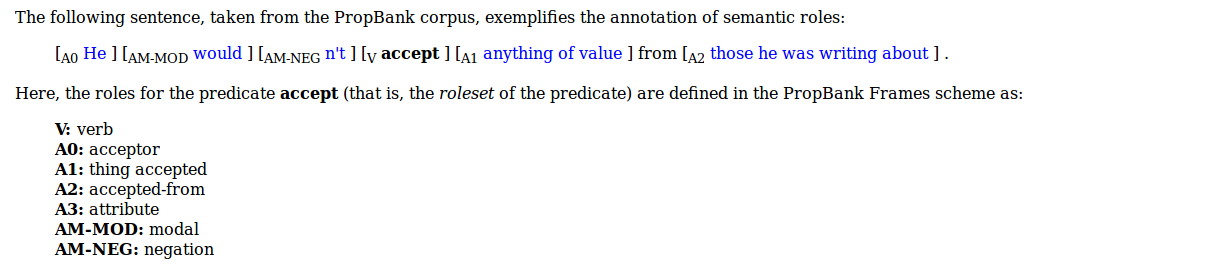
\includegraphics[width=\textwidth]{SRL.png}
\end{itemize}
\end{frame}

\begin{frame}
\frametitle{Midterm Preparation + Attendance}
\begin{itemize}
\item Form into your mid-term groups, work on your presentations for next week
\item Before you leave, post a 3 sentence summary of your presentation on Canvas, giving the team member names.  
\item That counts as your attendance for today.
\end{itemize}
\end{frame}

\begin{frame}
\frametitle{Next class}
\begin{itemize}
\item Conclusion of NLP Tasks overview
\item Quick introduction to machine learning and its relevance for language processing
\item Assignment 4 description
\item Instructions for mid-terms
\item (Probably) time for mid-term preps. 
\end{itemize}
\end{frame}

\end{document}



